\documentclass[compress]{beamer}
\usepackage{irbookslide}
\usepackage{irilmenau2}
\usepackage{tikz}
\usepackage{url}
\usepackage{ifxetex}
%\RequireXeTeX
\usepackage{fontspec} % zahteva paket euenc
\usepackage{xunicode}
\usepackage{xltxtra}
\usepackage{polyglossia}
\usepackage{minted}
\usepackage{algorithmic}
\renewcommand{\algorithmicrequire}{\textbf{Input:}}
\renewcommand{\algorithmicensure}{\textbf{Output:}}
\usepackage{xcolor,colortbl}
\usepackage{textcomp}
\usepackage{unicode-math}
%\setdefaultlanguage[script=Latin]{serbian}

\title{Stabla pretrage}
\author{\textcopyright \ \ Goodrich, Tamassia, Goldwasser}
\institute{Katedra za informatiku, Fakultet tehničkih nauka, Univerzitet u
Novom Sadu}
\date{2014.}
\subject{Predavanja sa ASP}

\begin{document}

\frame{\titlepage}

\section[Binarno stablo]{Binarno stablo pretrage}
\begin{frame}[fragile]
  \frametitle{Mape sa poretkom}
  \begin{itemize}
    \item postoji relacija poretka nad ključevima 
    \item elementi se skladište prema vrednosti ključa
    \item pretrage ,,najbliži sused`` (nearest neighbor):
    \begin{itemize}
      \item nađi element sa najvećim ključem manjim ili jednakim $k$
      \item nađi element sa najmanjim ključem većim ili jednakim $k$
    \end{itemize}
  \end{itemize}
\end{frame}

\begin{frame}[fragile]
  \frametitle{Binarna pretraga}
  \begin{itemize}
    \item binarna pretraga može da pronađe ,,najbližeg suseda`` za mapu sa poretkom implementiranu pomoću niza koji je sortiran po ključu 
    \begin{itemize}
      \item u svakom koraku prepolovi se broj kandidata
      \item radi u $O(\log n)$ vremenu
    \end{itemize}
    \item primer: nađi 7 
  \end{itemize}
  \begin{center}
    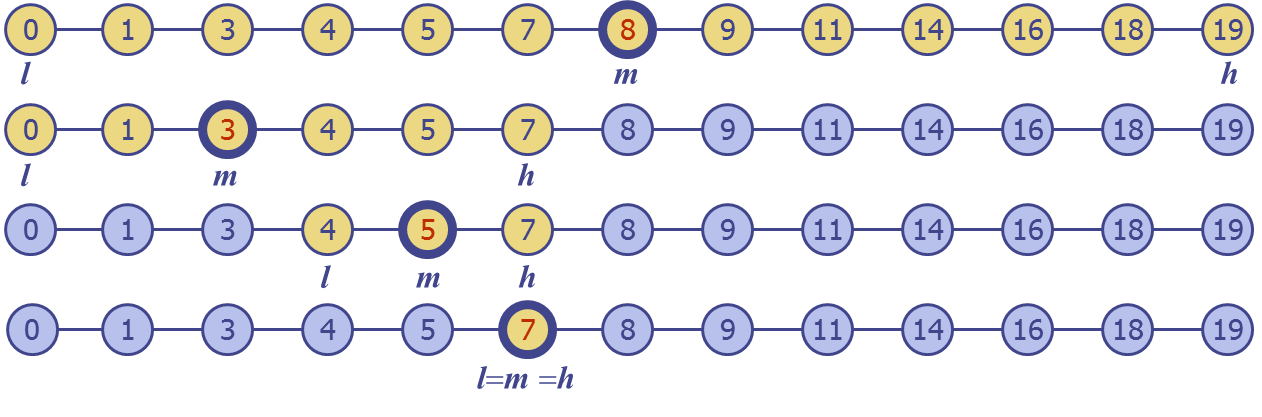
\includegraphics[width=10cm]{asp-11-pic01.png}
  \end{center}
\end{frame}

\begin{frame}[fragile]
  \frametitle{Tabela pretrage}
  \begin{itemize}
    \item tabela pretrage je mapa sa poretkom implementirana pomoću sortiranog niza 
    \begin{itemize}
      \item eksterni komparator za ključeve
    \end{itemize}
    \item performanse: 
    \begin{itemize}
      \item binarna pretraga je $O(\log n)$
      \item dodavanje je $O(n)$
      \item uklanjanje je $O(n)$
    \end{itemize}
    \item radi efikasno samo za mali broj elemenata ili tamo gde je pretraga česta a izmene retke (npr. provera kreditne kartice) 
  \end{itemize}
\end{frame}

\begin{frame}[fragile]
  \frametitle{Sortirana mapa ATP}
  \begin{itemize}
    \item standardne operacije mape 
  \end{itemize}
  \begin{center}
    \begin{tabular}{rp{8cm}}
      \textbf{\texttt{M[k]}} & vraća vrednost $v$ za ključ $k$ u mapi $M$; implementira je \texttt{\_\_getitem\_\_} \\ \hline
      \textbf{\texttt{M[k]=v}} & dodaje novi element $(k, v)$ u $M$ ili menja postojeći; implementira je \texttt{\_\_setitem\_\_} \\ \hline
      \textbf{\texttt{del M[k]}} & uklanja element sa ključem $k$ iz $M$; implementira je \texttt{\_\_delitem\_\_} \\
    \end{tabular}
  \end{center}
  \begin{itemize}
    \item dodatne funkcionalnosti 
    \begin{itemize}
      \item sortiran redosled prilikom iteracije
      \item nađi veće: \myred{find\_gt}($k$)
      \item nađi u opsegu: \myred{find\_range}($start, stop$) 
    \end{itemize}
  \end{itemize}
\end{frame}

\begin{frame}[fragile]
  \frametitle{Binarno stablo pretrage}
  \begin{itemize}
    \item \myred{binarno stablo pretrage} je binarno stablo koje čuva $(k, v)$ parove u čvorovima $p$ tako da važi:
    \begin{itemize}
      \item ključevi koji se nalaze u \textbf{levom} podstablu od $p$ su \textbf{manji} od $k$
      \item ključevi koji se nalaze u \textbf{desnom} podstablu od $p$ su \textbf{veći} od $k$
    \end{itemize}
    \item listovi ne čuvaju elemente, reference na listove mogu biti None
    \item inorder obilazak: ključevi u rastućem redosledu 
  \end{itemize}
  \begin{center}
    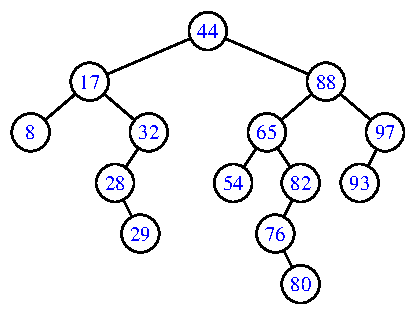
\includegraphics[width=6cm]{asp-11-pic02.pdf}
  \end{center}
\end{frame}

\begin{frame}[fragile]
  \frametitle{Pretraga u binarnom stablu}
  \begin{itemize}
    \item tražimo ključ $k$ polazeći od korena
    \item idemo levo ako je $k$ manji od tekućeg čvora
    \item idemo desno ako je $k$ veći od tekućeg čvora
    \item ako dođemo do lista, $k$ nije nađen
  \end{itemize}
  \begin{columns}
    \begin{column}[c]{6cm}
      \begin{center}
        Tražimo 65
        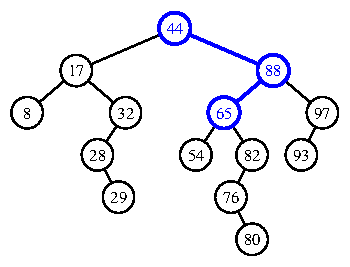
\includegraphics[width=6cm]{asp-11-pic03a.pdf}
      \end{center}
    \end{column}  
    \begin{column}[c]{6cm}
      \begin{center}
        Tražimo 68
        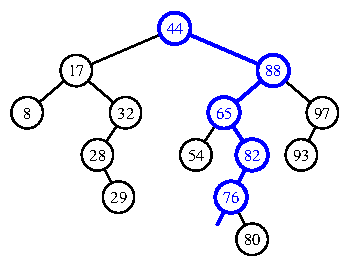
\includegraphics[width=6cm]{asp-11-pic03b.pdf}
      \end{center}
    \end{column}  
  \end{columns}
\end{frame}

\renewcommand{\algorithmiccomment}[1]{\hfill \{\myred{#1}\}}

\begin{frame}[fragile]
  \frametitle{Pretraga u binarnom stablu}
\myred{TreeSearch}($T, p, k$)
\begin{algorithmic}
\IF{$k = p.key$}
  \RETURN $p$ \COMMENT{pronađen}
\ELSIF{$k < p.key \land T.left(p) \neq None$}
  \RETURN TreeSearch($T, T.left(p), k$) \COMMENT{levo podstablo}
\ELSIF{$k > p.key \land T.right(p) \neq None$}
  \RETURN TreeSearch($T, T.right(p), k$) \COMMENT{desno podstablo}
\ENDIF
\RETURN None  \COMMENT{nije pronađen}
\end{algorithmic}
\end{frame}

\begin{frame}[fragile]
  \frametitle{Performanse pretrage u binarnom stablu}
  \begin{itemize}
    \item u svakom rekurzivnom pozivu spuštamo se za jedan nivo u stablu
    \item testiranje u okviru jednog nivoa je $O(1)$
    \item ukupan broj testova je $O(h)$, gde je $h$ visina stabla
  \end{itemize}
  \begin{center}
    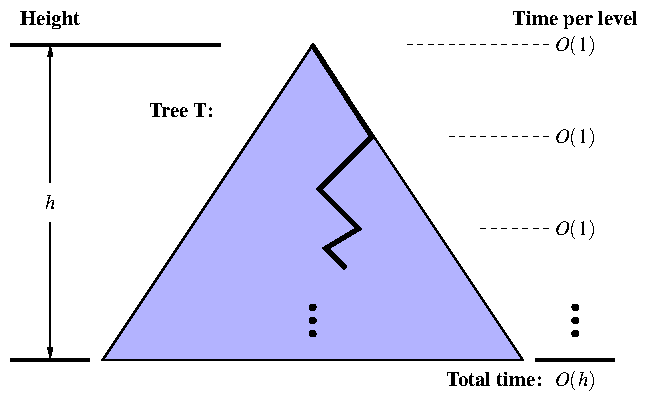
\includegraphics[width=8cm]{asp-11-pic04.pdf}
  \end{center}
\end{frame}

\begin{frame}[fragile]
  \frametitle{Dodavanje u stablo}
  \begin{itemize}
    \item dodajemo element $(k, v)$
    \item prvo tražimo $k$
    \item ako $k$ nije u stablu, došli smo do lista gde treba dodati čvor
    \item primer: dodajemo 68
  \end{itemize}
  \begin{columns}
    \begin{column}[c]{6cm}
      \begin{center}
        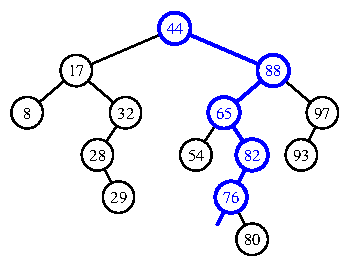
\includegraphics[width=6cm]{asp-11-pic05a.pdf}
      \end{center}
    \end{column}  
    \begin{column}[c]{6cm}
      \begin{center}
        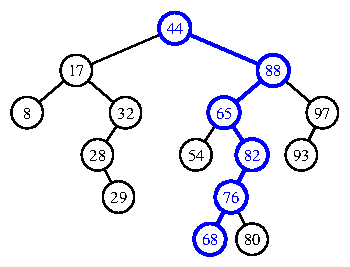
\includegraphics[width=6cm]{asp-11-pic05b.pdf}
      \end{center}
    \end{column}  
  \end{columns}
\end{frame}

\begin{frame}[fragile]
  \frametitle{Dodavanje u stablo}
\myred{TreeInsert}($T, k, v$)
\begin{algorithmic}
\STATE $p \leftarrow$ TreeSearch($T, T.root, k$)
\IF{$k = p.key$}
  \STATE $p.value \leftarrow v$  \COMMENT{ako već postoji zameni vrednost}
\ELSIF{$k < p.key$}
  \STATE $p$.add\_left($k, v$) \COMMENT{dodaj levo dete}
\ELSE
  \STATE $p$.add\_right($k, v$) \COMMENT{dodaj desno dete}
\ENDIF
\end{algorithmic}
  \begin{itemize}
    \item dodaje se uvek u list
  \end{itemize}
\end{frame}

\begin{frame}[fragile]
  \frametitle{Uklanjanje iz stabla}
  \begin{itemize}
    \item uklanjamo element sa ključem $k$
    \item prvo nađemo $p$ koji sadrži $k$
    \item ako $p$ ima \textbf{najviše jedno} dete
    \item njegovo dete $r$ vežemo u stablo umesto njega
    \item primer: uklanjamo 32
  \end{itemize}
  \begin{columns}
    \begin{column}[c]{6cm}
      \begin{center}
        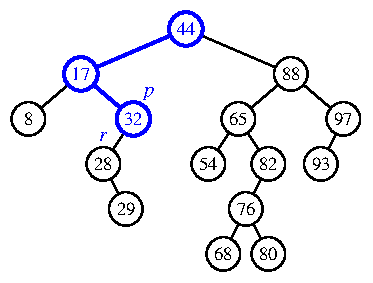
\includegraphics[width=6cm]{asp-11-pic06a.pdf}
      \end{center}
    \end{column}  
    \begin{column}[c]{6cm}
      \begin{center}
        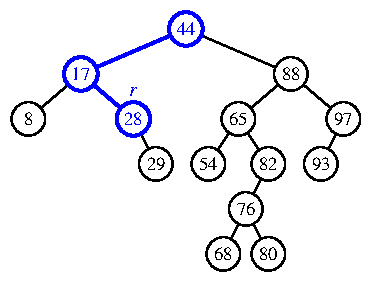
\includegraphics[width=6cm]{asp-11-pic06b.pdf}
      \end{center}
    \end{column}  
  \end{columns}
\end{frame}

\begin{frame}[fragile]
  \frametitle{Uklanjanje iz stabla}
  \begin{itemize}
    \item ako $p$ ima \textbf{dva} deteta
    \begin{itemize}
      \item nađemo čvor $r$ čiji ključ neposredno prethodi $p$ -- to je ,,najdesniji`` čvor u njegovom levom podstablu
      \item vežemo $r$ na mesto $p$; pošto $r$ neposredno prethodi $p$ po vrednosti ključa, svi elementi u desnom podstablu od $p$ su veći od $r$ i svi elementi u levom podstablu od $p$ su manji od $r$
      \item treba još obrisati stari $r$ -- pošto je to ,,najdesniji`` element, on nema desno dete, pa se može obrisati po prethodnom algoritmu
    \end{itemize}
    \item primer: uklanjamo 88
  \end{itemize}
  \begin{columns}
    \begin{column}[c]{6cm}
      \begin{center}
        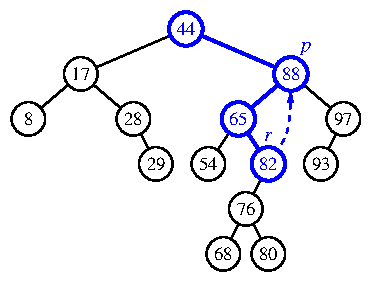
\includegraphics[width=4.5cm]{asp-11-pic07a.pdf}
      \end{center}
    \end{column}  
    \begin{column}[c]{6cm}
      \begin{center}
        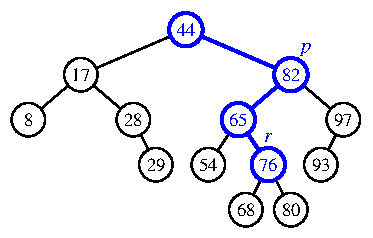
\includegraphics[width=4.5cm]{asp-11-pic07b.pdf}
      \end{center}
    \end{column}  
  \end{columns}
\end{frame}

\begin{frame}[fragile]
  \frametitle{Performanse binarnog stabla pretrage}
  \begin{columns}
    \begin{column}[c]{6cm}
      \begin{itemize}
        \item zauzeće memorije je $O(n)$
        \item pretraga, dodavanje i uklanjanje su $O(h)$
        \item visina stabla $h$ je $O(\log n) \leq h \leq O(n)$
      \end{itemize}
    \end{column}  
    \begin{column}[c]{6cm}
      \begin{center}
        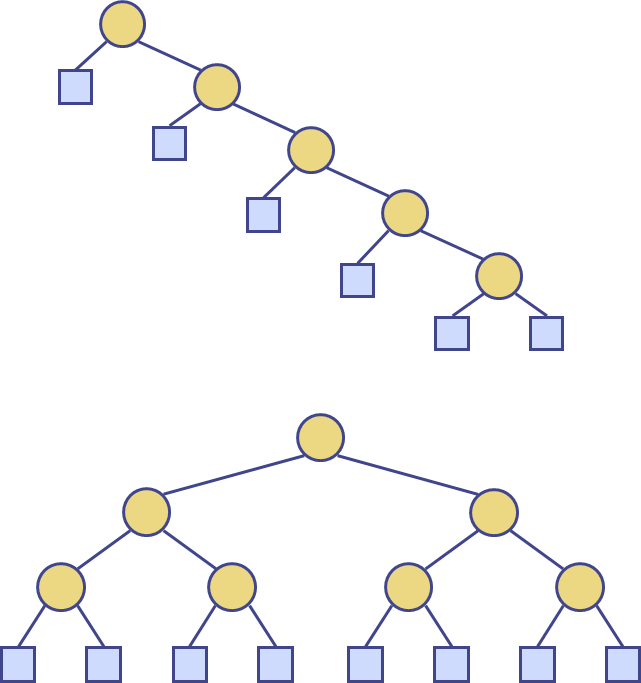
\includegraphics[width=5cm]{asp-11-pic08.png}
      \end{center}
    \end{column}  
  \end{columns}
  \\ \ \\ \hfill balansirano stablo ima bolje performanse
\end{frame}

\section[Balansiranje]{Balansiranje binarnog stabla}
\begin{frame}[fragile]
  \frametitle{Balansiranje binarnog stabla}
  \begin{itemize}
    \item osnovna operacija za balansiranje je \myred{rotacija}
    \item ,,rotiramo`` dete i njegovog roditelja
    \item tom prilikom i podstabla menjaju mesta
    \item jedna rotacija traje $O(1)$
  \end{itemize}
  \begin{center}
    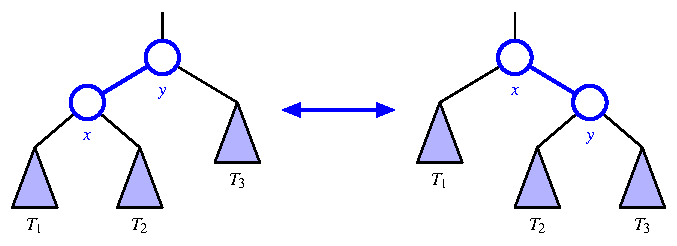
\includegraphics[width=10cm]{asp-11-pic09.pdf}
  \end{center}
\end{frame}

\begin{frame}[fragile]
  \frametitle{Balansiranje binarnog stabla}
  \begin{itemize}
    \item kompozitna operacija ,,\myred{restrukturiranje tri čvora}`` (tri-node restructuring)
    \item posmatraju se čvor, njegovo dete i unuče
    \item cilj je da se skrati putanja od čvora do unučeta
    \item četiri moguća rasporeda čvorova
    \begin{itemize}
      \item prva dva traže jednu rotaaciju
      \item druga dva traže dve rotacije
    \end{itemize}
  \end{itemize}
\end{frame}

\begin{frame}[fragile]
  \frametitle{Restrukturiranje sa jednom rotacijom}
  \begin{center}
    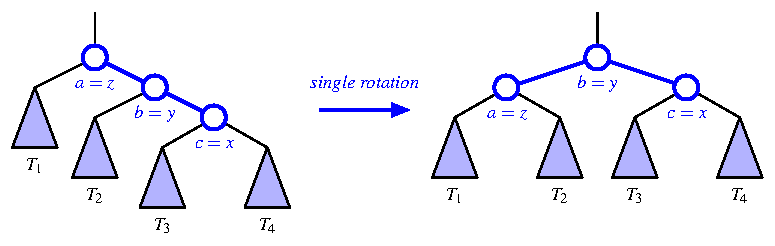
\includegraphics[width=10cm]{asp-11-pic10.pdf}
  \end{center}
  \begin{center}
    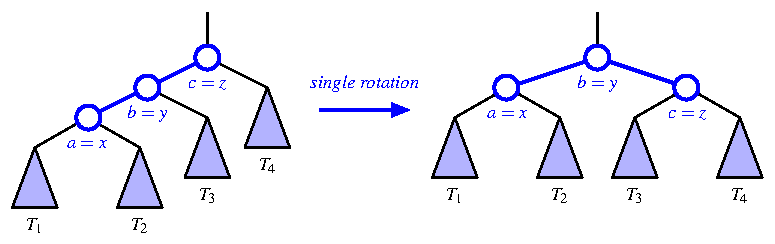
\includegraphics[width=10cm]{asp-11-pic11.pdf}
  \end{center}
\end{frame}

\begin{frame}[fragile]
  \frametitle{Restrukturiranje sa dve rotacije}
  \begin{center}
    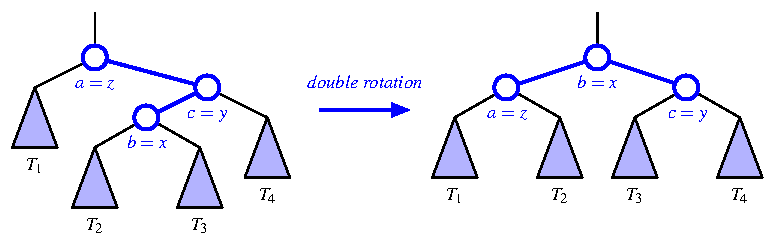
\includegraphics[width=10cm]{asp-11-pic12.pdf}
  \end{center}
  \begin{center}
    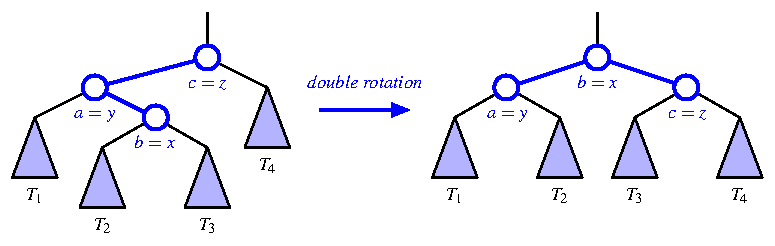
\includegraphics[width=10cm]{asp-11-pic13.pdf}
  \end{center}
\end{frame}

\section[AVL stablo]{AVL stablo}

\begin{frame}[fragile]
  \frametitle{AVL stablo}
  \begin{itemize}
    \item autori: G.M. \myred{A}delson-\myred{V}elskii i E. \myred{L}andis
    \item visina podstabla: broj čvorova na najdužoj putanji od korena do lista
    \item visina čvora = visina podstabla sa njim kao korenom
    \item \myred{AVL stablo} je binarno stablo koje ima dodatnu osobinu:
    \begin{itemize}
      \item za svaki čvor u stablu, visine njegove dece razlikuju se najviše za 1
    \end{itemize}
  \end{itemize}
  \begin{center}
    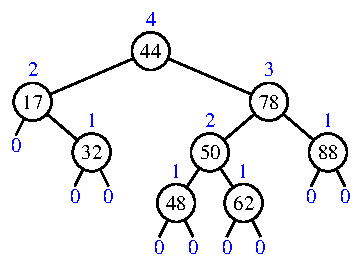
\includegraphics[width=5cm]{asp-11-pic14.pdf}
  \end{center}
\end{frame}

\begin{frame}[fragile]
  \frametitle{Visina AVL stabla}
  \begin{itemize}
    \item \textbf{teorema}: visina AVL stabla sa $n$ čvorova je $O(\log n)$
    \item \textbf{dokaz}: $n(h)$ -- najmanji broj unutrašnjih čvorova u AVL stablu visine $h$
    \item očevidno: $n(1)=1$, $n(2)=2$
    \item za $n>2$, AVL stablo visine $h$ sadrži koren, podstablo visine $h-1$ i podstablo visine $h-2$
    \item tj. $n(h) = 1 + n(h-1) + n(h-2)$
    \item kako je $n(h-1)>n(h-2)$, važi $n(h)>2n(h-2)$
    \begin{itemize}
      \item indukcijom: $n(h)>2n(h-2)$, $n(h)>4n(h-4)$, $n(h)>8(h-6)$, \ldots
      \item \myred{$n(h)>2^in(h-2i)$}
    \end{itemize}
    \item bazni slučaj: $n(h)>2^{h/2-1}$
    \item odnosno: $h < 2\log n(h) + 2$
    \item tj. visina AVL stabla $h$ je $O(\log n)$
  \end{itemize}
\end{frame}

\begin{frame}[fragile]
  \frametitle{AVL stablo: dodavanje}
  \begin{itemize}
    \item stablo u koje dodajemo novi čvor je AVL stablo
    \item dodavanje se vrši isto kao kod binarnog stabla -- u list
    \item dodavanje može da naruši balansiranost
    \item čvorovi koji mogu biti disbalansirani su samo preci novog čvora
    \item primer: dodajemo čvor 54
  \end{itemize}
  \begin{columns}
    \begin{column}[t]{6cm}
      \begin{center}
        pre balansiranja 
        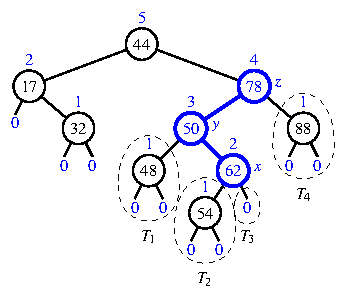
\includegraphics[width=5cm]{asp-11-pic15a.pdf}
      \end{center}
    \end{column}  
    \begin{column}[t]{6cm}
      \begin{center}
        posle balansiranja
        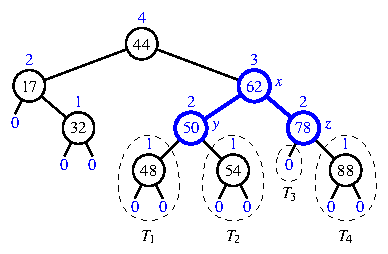
\includegraphics[width=6cm]{asp-11-pic15b.pdf}
      \end{center}
    \end{column}  
  \end{columns}
\end{frame}

\begin{frame}[fragile]
  \frametitle{AVL stablo: dodavanje}
  \begin{itemize}
    \item ,,search-and-repair`` strategija
    \item $z$ -- prvi nebalansirani čvor na polazeći od $p$ koji smo naišli
    %\item $y$ -- dete $z$ sa većom visinom (takođe predak $p$)
    %\item $y$ -- dete $y$ sa većom visinom (predak $p$ ili sâm $p$)
    \item radimo \textbf{trinode restructuring} za $z$ 
  \end{itemize}
  \begin{columns}
    \begin{column}[t]{6cm}
      \begin{center}
        pre balansiranja 
        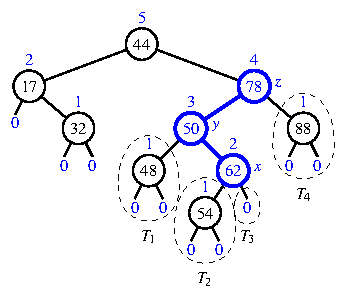
\includegraphics[width=5cm]{asp-11-pic15a.pdf}
      \end{center}
    \end{column}  
    \begin{column}[t]{6cm}
      \begin{center}
        posle balansiranja
        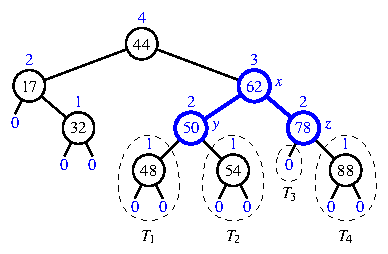
\includegraphics[width=6cm]{asp-11-pic15b.pdf}
      \end{center}
    \end{column}  
  \end{columns}
\end{frame}

\begin{frame}[fragile]
  \frametitle{AVL stablo: dodavanje}
pre dodavanja: 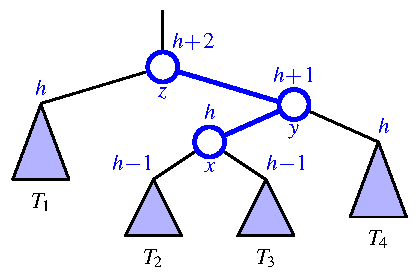
\includegraphics[width=3.5cm]{asp-11-pic16a.pdf}

dodavanje u $T_3$ remeti balans u $z$: 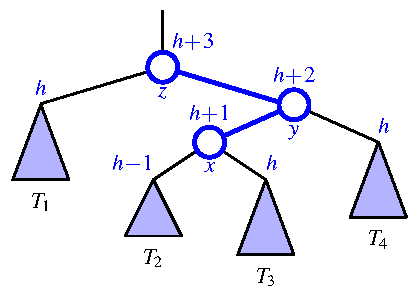
\includegraphics[width=3.5cm]{asp-11-pic16b.pdf}

nakon restrukturiranja: 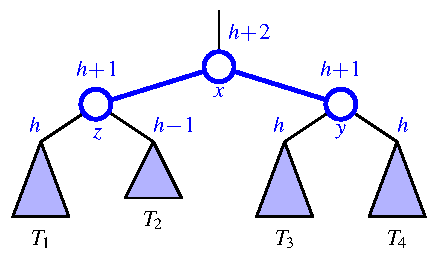
\includegraphics[width=3.5cm]{asp-11-pic16c.pdf}
\end{frame}

\begin{frame}[fragile]
  \frametitle{AVL stablo: uklanjanje}
  \begin{itemize}
    \item uklanja se uvek čvor koji ima 0 ili 1 dete
    \item time se može narušiti balans AVL stabla
    \item i ovde radimo restrukturiranje posle uklanjanja
    \item primer: uklanjamo 32
  \end{itemize}
  \begin{columns}
    \begin{column}[t]{6cm}
      \begin{center}
        pre balansiranja, koren nije balansiran 
        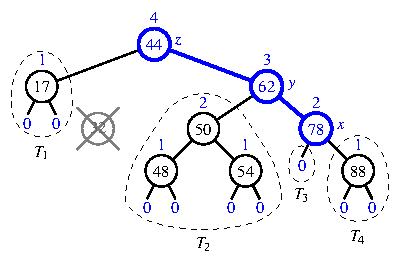
\includegraphics[width=5cm]{asp-11-pic17a.pdf}
      \end{center}
    \end{column}  
    \begin{column}[t]{6cm}
      \begin{center}
        posle balansiranja (jedna rotacija)
        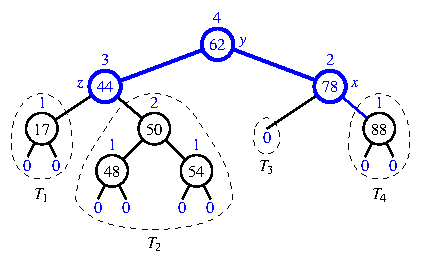
\includegraphics[width=6cm]{asp-11-pic17b.pdf}
      \end{center}
    \end{column}  
  \end{columns}
\end{frame}

\begin{frame}[fragile]
  \frametitle{AVL stablo: performanse}
  \begin{itemize}
    \item jedno restrukturiranje je $O(1)$ 
    \item pretraga je $O(\log n)$ -- visina stabla je $O(\log n)$
    \item dodavanje je $O(\log n)$
    \begin{itemize}
      \item pronalaženje mesta je $O(\log n)$
      \item restrukturiranje uz stablo je $O(\log n)$
    \end{itemize}
    \item uklanjanje je $O(\log n)$
    \begin{itemize}
      \item pronalaženje mesta je $O(\log n)$
      \item restrukturiranje uz stablo je $O(\log n)$
    \end{itemize}
  \end{itemize}
\end{frame}

\section[Splay stablo]{Splay stablo}
\begin{frame}[fragile]
  \frametitle{Splay stablo}
  \begin{itemize}
    \item \myred{splay}: ,,rašireno`` 
    \item ne nameće logaritamsko ograničenje na visinu
    \item \myred{splaying}: ,,širenje`` stabla prilikom dodavanja, uklanjanja \textbf{i pretrage}
    \item ideja: da češće korišćeni elementi budu bliže korenu
  \end{itemize}
\end{frame}

\begin{frame}[fragile]
  \frametitle{Splaying}
  \begin{itemize}
    \item čvor $x$ se premešta u koren nizom restrukturiranja 
    \item operacije restrukturiranja zavise od položaja $x$, $y$ (roditelja) i $z$ (dede, ako postoji)
    \item postoje tri slučaja:
    \begin{itemize}
      \item \myred{zig-zig}
      \item \myred{zig-zag}
      \item \myred{zig}
    \end{itemize}
  \end{itemize}
\end{frame}

\begin{frame}[fragile]
  \frametitle{Splaying: zig-zig}
  \begin{itemize}
    \item $x$ i $y$ su  
    \begin{itemize}
      \item obojica levo dete svog roditelja ili
      \item obojica desno dete svog roditelja
    \end{itemize}
    \item $x$ postaje koren, $y$ njegovo dete, $z$ njegovo unuče
  \end{itemize}
  \begin{columns}
    \begin{column}[t]{6cm}
      \begin{center}
        pre zig-zig 
        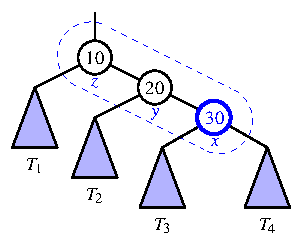
\includegraphics[width=5cm]{asp-11-pic18a.pdf}
      \end{center}
    \end{column}  
    \begin{column}[t]{6cm}
      \begin{center}
        posle zig-zig
        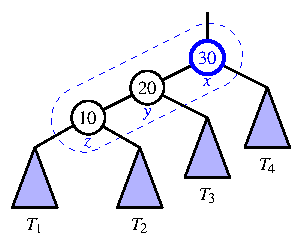
\includegraphics[width=5cm]{asp-11-pic18b.pdf}
      \end{center}
    \end{column}  
  \end{columns}
\end{frame}

\begin{frame}[fragile]
  \frametitle{Splaying: zig-zag}
  \begin{itemize}
    \item $x$ i $y$ 
    \begin{itemize}
      \item prvi je levo dete a drugi je desno dete, ili
      \item prvi je desno dete a drugi je levo dete
    \end{itemize}
    \item $x$ postaje koren, $y$ i $z$ njegova deca
  \end{itemize}
  \begin{columns}
    \begin{column}[t]{6cm}
      \begin{center}
        pre zig-zag 
        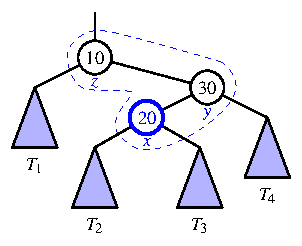
\includegraphics[width=5cm]{asp-11-pic19a.pdf}
      \end{center}
    \end{column}  
    \begin{column}[t]{6cm}
      \begin{center}
        posle zig-zag
        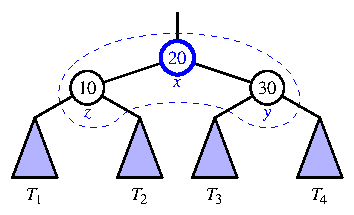
\includegraphics[width=6cm]{asp-11-pic19b.pdf}
      \end{center}
    \end{column}  
  \end{columns}
\end{frame}

\begin{frame}[fragile]
  \frametitle{Splaying: zig}
  \begin{itemize}
    \item $x$ ima roditelja $y$ ali nema dedu $z$ \ \ :(
    \item $x$ postaje koren, $y$ njegovo dete
  \end{itemize}
  \begin{columns}
    \begin{column}[t]{6cm}
      \begin{center}
        pre zig
        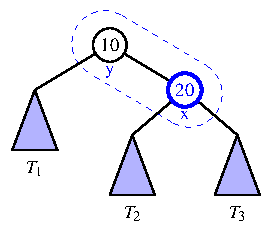
\includegraphics[width=5cm]{asp-11-pic20a.pdf}
      \end{center}
    \end{column}  
    \begin{column}[t]{6cm}
      \begin{center}
        posle zig
        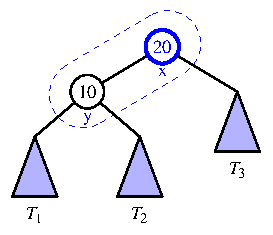
\includegraphics[width=5cm]{asp-11-pic20b.pdf}
      \end{center}
    \end{column}  
  \end{columns}
\end{frame}

\begin{frame}[fragile]
  \frametitle{Splaying: primer $_1$}
  \begin{itemize}
    \item zig-zig, zig-zag i zig primenjujemo sve dok $x$ ne postane koren
    \item primer: dodajemo 14
    \item na 14 se primenjuje zig-zag (jer 14 je desno dete a 13 je levo dete)
  \end{itemize}
  \begin{center}
    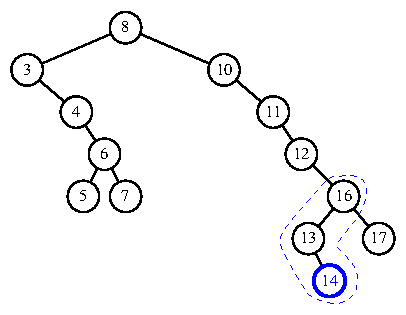
\includegraphics[width=7cm]{asp-11-pic21.pdf}
  \end{center}
\end{frame}

\begin{frame}[fragile]
  \frametitle{Splaying: primer $_2$}
  \begin{itemize}
    \item posle primenjenog zig-zag stanje je
  \end{itemize}
  \begin{center}
    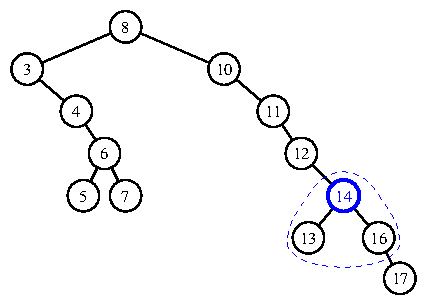
\includegraphics[width=7cm]{asp-11-pic22.pdf}
  \end{center}
\end{frame}

\begin{frame}[fragile]
  \frametitle{Splaying: primer $_3$}
  \begin{itemize}
    \item sada može da se primeni zig-zig
  \end{itemize}
  \begin{center}
    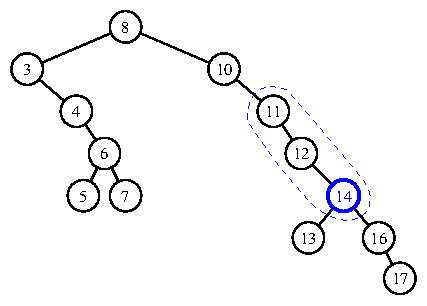
\includegraphics[width=7cm]{asp-11-pic23.pdf}
  \end{center}
\end{frame}

\begin{frame}[fragile]
  \frametitle{Splaying: primer $_4$}
  \begin{itemize}
    \item nakon primene zig-zig
  \end{itemize}
  \begin{center}
    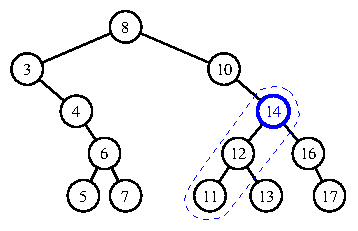
\includegraphics[width=7cm]{asp-11-pic24.pdf}
  \end{center}
\end{frame}

\begin{frame}[fragile]
  \frametitle{Splaying: primer $_5$}
  \begin{itemize}
    \item sada može ponovo zig-zig
  \end{itemize}
  \begin{center}
    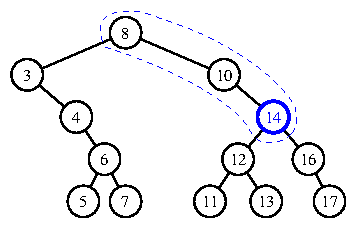
\includegraphics[width=7cm]{asp-11-pic25.pdf}
  \end{center}
\end{frame}

\begin{frame}[fragile]
  \frametitle{Splaying: primer $_6$}
  \begin{itemize}
    \item nakon drugog zig-zig
  \end{itemize}
  \begin{center}
    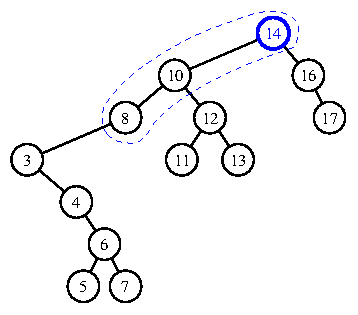
\includegraphics[width=7cm]{asp-11-pic26.pdf}
  \end{center}
\end{frame}

\begin{frame}[fragile]
  \frametitle{Splay stablo: performanse}
  \begin{itemize}
    \item zig-zig, zig-zag i zig su $O(1)$
    \item splaying čvora $p$ je $(d)$ gde je $d$ dubina čvora $p$
    \item tj. isto koliko je potrebno i za navigaciju od korena do $p$ \\ \ \\
    \item u najgorem slučaju, pretraga, dodavanje i uklanjanje su $O(h)$ gde je $h$ visina stabla
    \item stablo nije balansirano $\Rightarrow$ može biti $h=n$
    \item $\Rightarrow$ slabe performanse u najgorem slučaju
  \end{itemize}
\end{frame}

\begin{frame}[fragile]
  \frametitle{Splay stablo: performanse}
  \begin{itemize}
    \item za \textbf{amortizovane} operacije vreme je $O(\log n)$
    \item a za često tražene podatke pretraga je i \textbf{brža od} $O(\log n)$
  \end{itemize}
\end{frame}

\end{document}